\subsection{Setup initial}

Toute cette partie est couverte par la formation précédente. Normalement, à la suite de tutoriel, vous devriez avoir obtenu le site suivant en vous rendant sur \url{http://lurlquevousavezchoisie}:\footnote{\underline{PS:}n'oubliez pas de lancer \verb|sail up -d| et \verb|sail npm run dev| si cela n'est pas déjà fait! Ne vous inquiétez pas, l'explication pour la deuxième commande va bientôt arriver\ldots}.

\begin{figure}[!h]
    \centering
    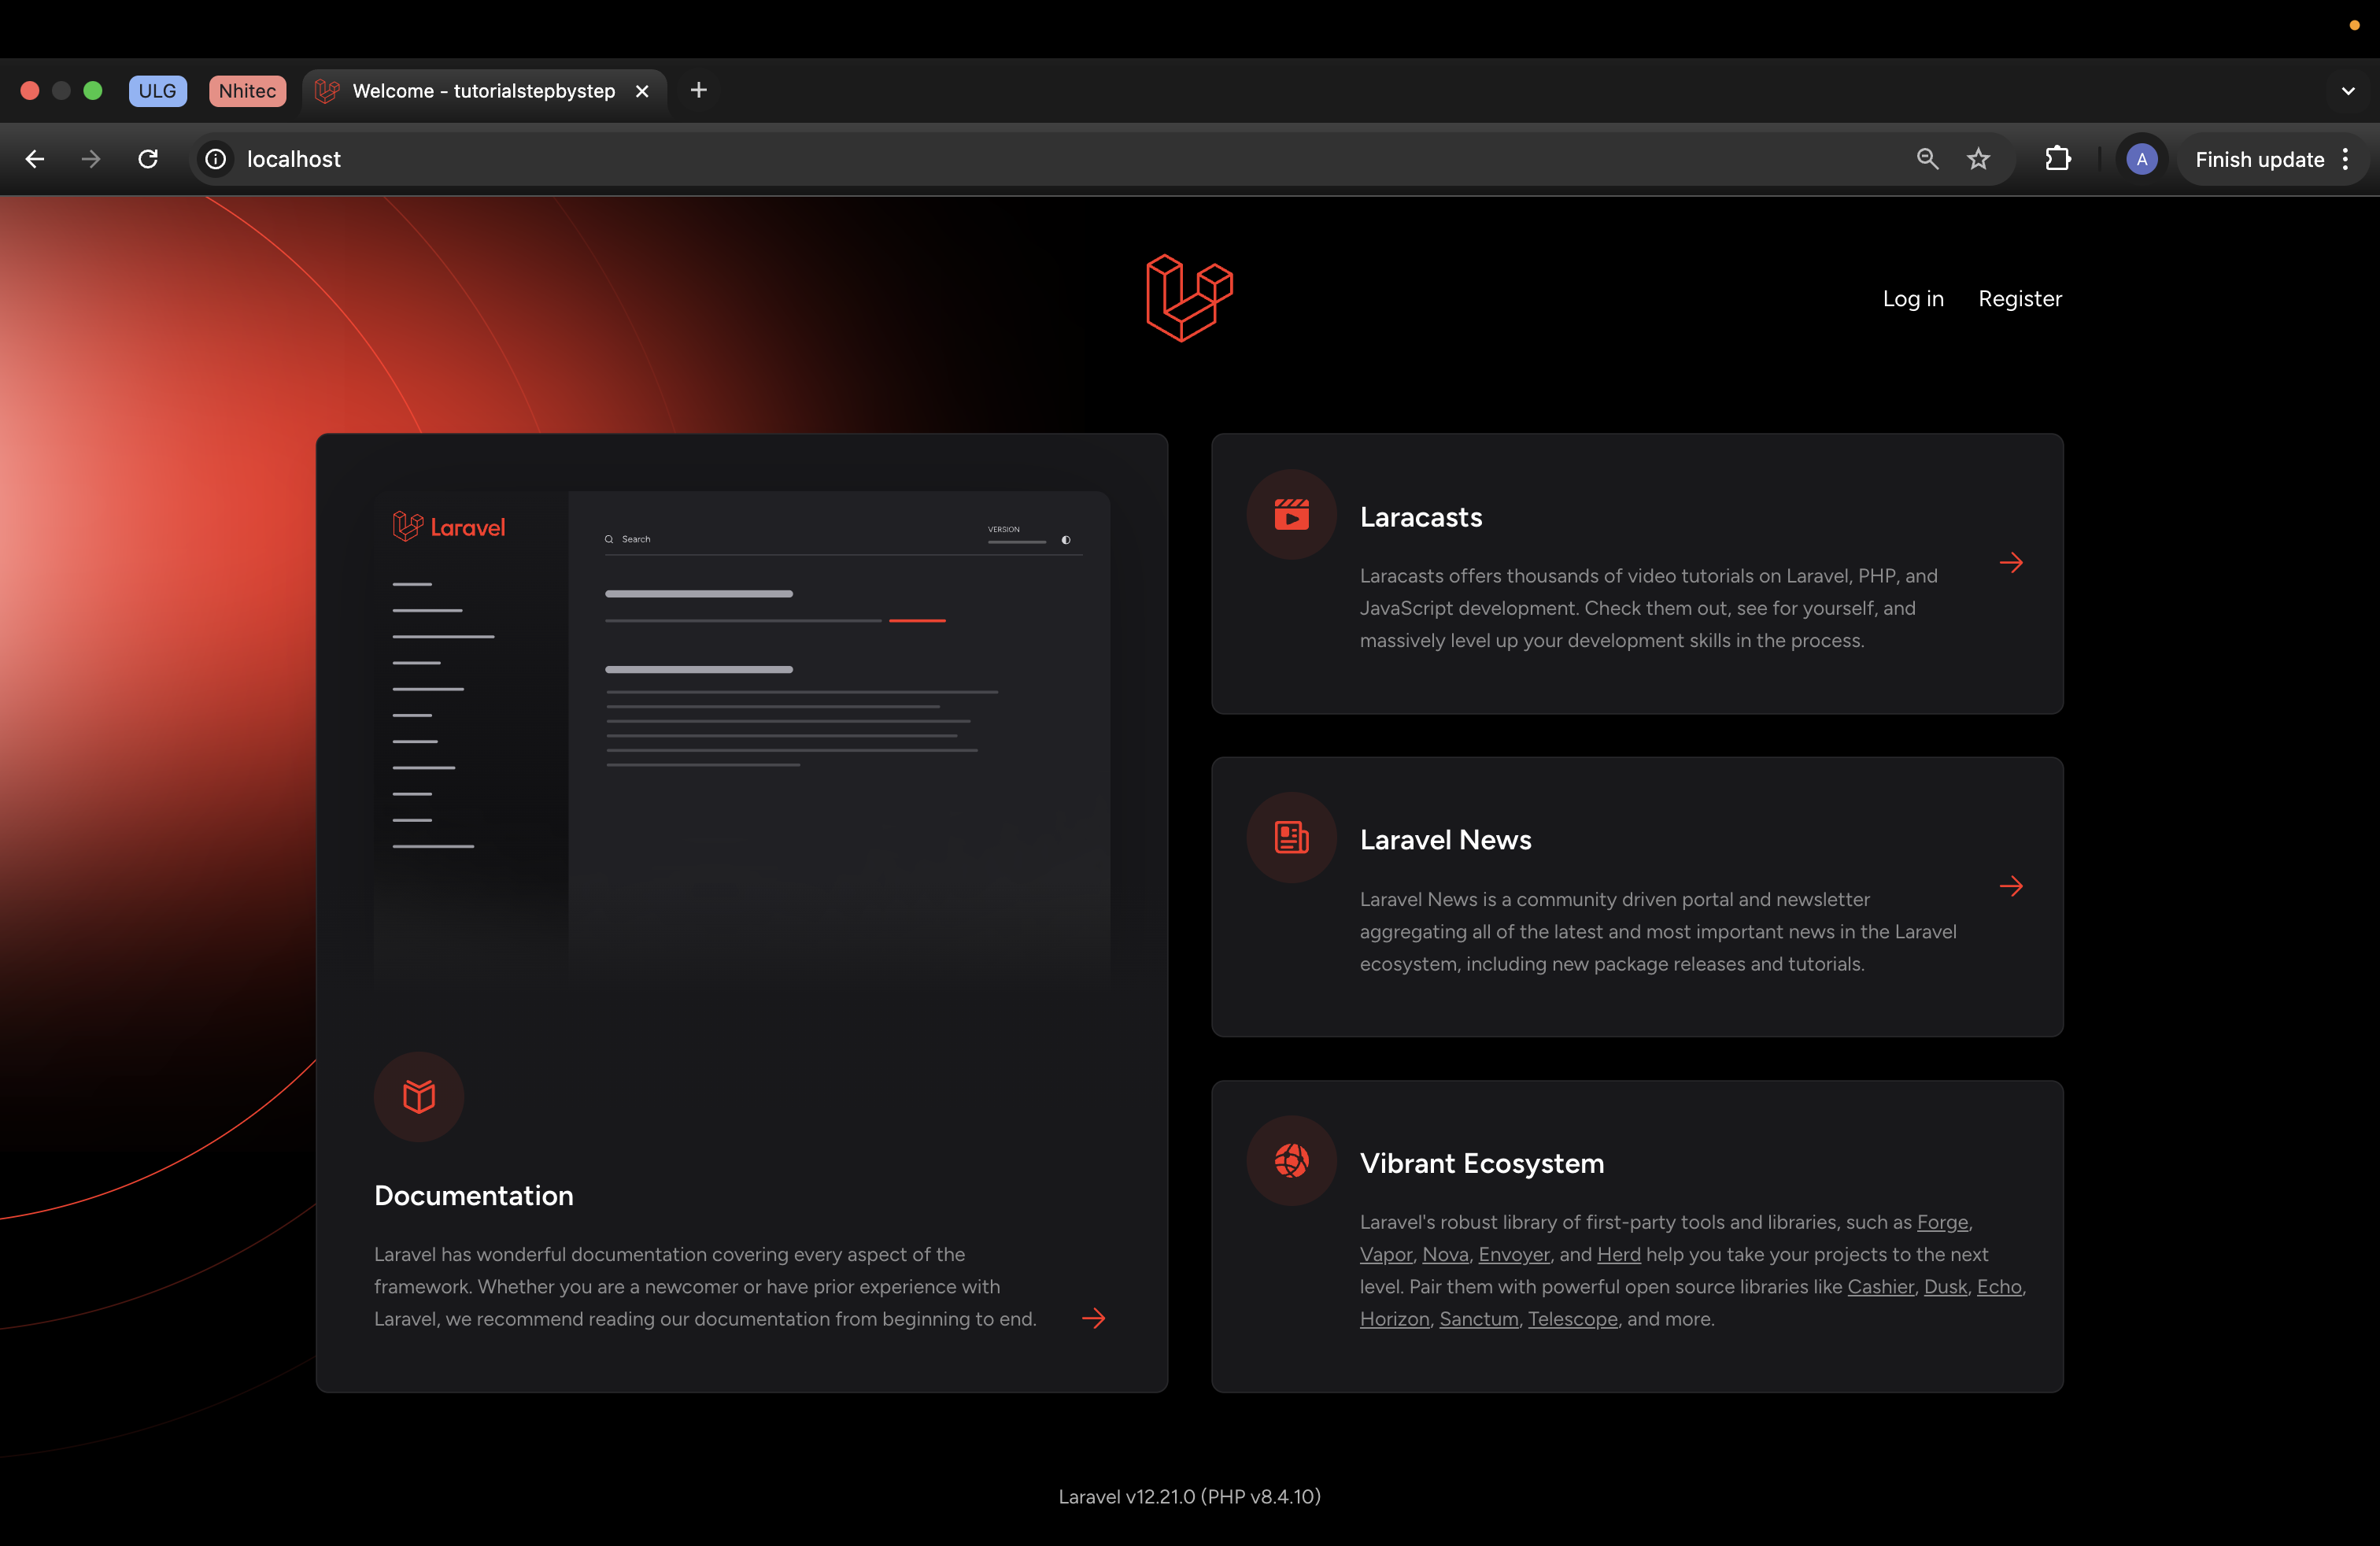
\includegraphics[width=0.75\textwidth]{figures-C1/laravel_default_website.png}
\end{figure}

Nous allons partir de ce site là. Pour ce tutoriel, mon projet sera appellé \texttt{tutorialstepbystep} donc son URL sera \url{http://tutorialstepbystep/}.

\newpage
\subsubsection[Extensions]{Extensions}

Vous allez rapidement remarquer de nouvelles fonctionnalités que mon IDE\footnote{Au cas où ça ne serait toujours pas clair, utilisez \vscode{} !!} possède par rapport au vôtre. Ces fonctionnalités sont rajoutées grâce aux extensions de \vscode{}. 

Pour éviter d’installer les extensions une par une, nous avons regroupé toutes les extensions utiles dans un pack unique.  

\begin{itemize}
    \item Ouvrez \vscode{}.
    \item Allez dans l’onglet \verb|Extensions| dans la barre d’outils à gauche.
    \item Recherchez \textbf{\texttt{N-HiTec - Op\&Ex Basic Extensions}}.
    \item Cliquez sur \textbf{Install}.
\end{itemize}

\begin{center}
    
\includegraphics[width=0.8\textwidth]{figures-C1/nhitecpack.png}
\end{center}

Grâce à ce pack, vous aurez directement un environnement de travail complet et prêt pour le développement.